\documentclass[10pt, conference, letterpaper]{IEEEtran}

\usepackage{graphicx}
\graphicspath{ {output/} }

\usepackage[subrefformat=parens,labelformat=parens,farskip=0pt]{subfig}
\usepackage[english]{babel}
\usepackage{blindtext}

\newcommand{\vsubfloat}[1]{%
\bgroup%
\renewcommand{\arraystretch}{0}%
\subfloat{\begin{tabular}[b]{@{}l@{}}#1\end{tabular}}%
\egroup%
}

\begin{document}
\begin{figure}[t]
\centering
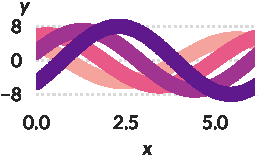
\includegraphics{plorts-halfcol}
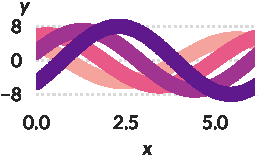
\includegraphics{plorts-halfcol}
\end{figure}
\begin{figure}
\centering
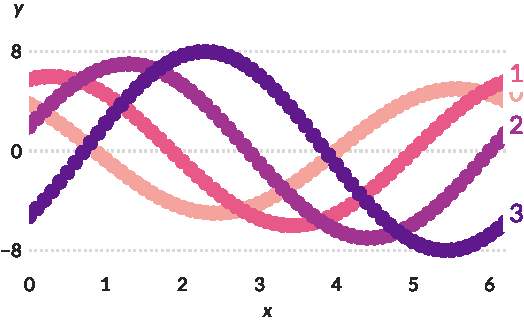
\includegraphics{plorts-col}
\end{figure}

\Blindtext

\begin{figure}[t]
  \centering
  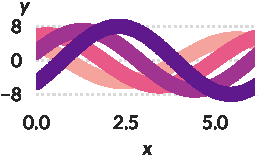
\includegraphics{plorts-halfcol}
  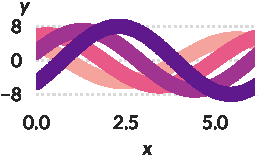
\includegraphics{plorts-halfcol}
\end{figure}
\begin{figure}
  \centering
  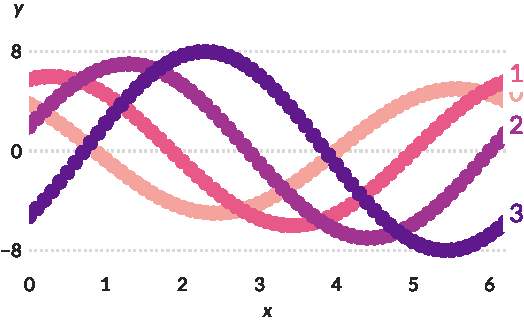
\includegraphics{plorts-col}
\end{figure}

\begin{figure*}
\centering
\subfloat{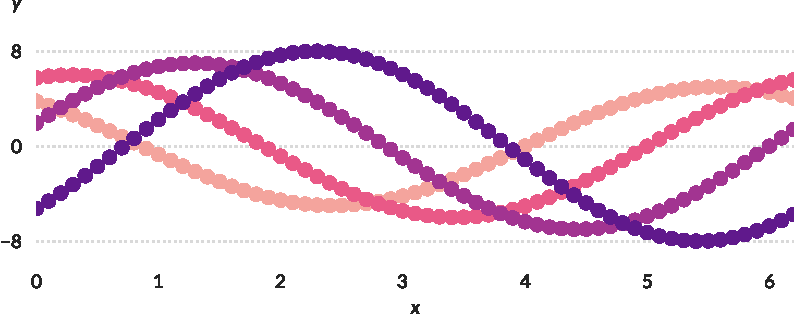
\includegraphics{plorts-onehalfcol}}
\hspace{\fill}
\vsubfloat{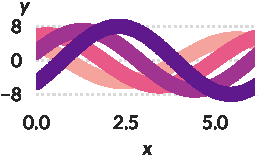
\includegraphics{plorts-halfcol}\\%
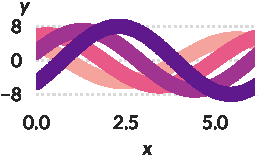
\includegraphics{plorts-halfcol}}%
\\
\subfloat{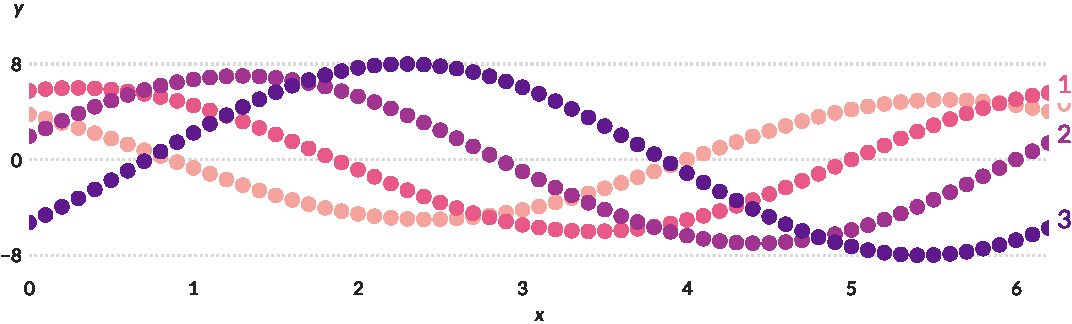
\includegraphics{plorts-twocol}}
\end{figure*}
\end{document}

%%% Local Variables:
%%% mode: latex
%%% TeX-master: t
%%% End:
